\documentclass[english,a4paper,hidelinks,pdftex, 11 pt, class=report,crop=false]{standalone}
\usepackage[T1]{fontenc}
\usepackage[utf8]{luainputenc}
\usepackage{geometry}
\setlength{\parindent}{0bp}
\usepackage{import}
\usepackage[subpreambles=false]{standalone}
\usepackage{amsmath}
\usepackage{amssymb}
\usepackage{esint}
\usepackage{babel}
\usepackage{tabu}
\usepackage{lmodern}
\usepackage[dvipsnames]{xcolor}
\geometry{verbose, inner=2.3cm, outer=1.8 cm, bmargin=2cm, tmargin=1.8cm}
% Lister med bokstavar
\usepackage{enumitem}

\newcommand{\os}{\\[5pt]}
\newcommand{\vsk}{\\[12pt]}
\newcommand{\net}[2]{{\href{#1}{\color{blue}#2}}}

\usepackage{bm}

\usepackage{hyperref}


\usepackage[many]{tcolorbox}
\newcommand{\reg}[2][]{\begin{tcolorbox}[boxrule=0.3 mm,arc=0mm,colback=blue!3] {\Large \textbf{#1} \vspace{5 pt}}\newline #2  \end{tcolorbox}\vspace{-5pt}}

\newcommand\eks[2][]{\begin{tcolorbox}[boxrule=0.3 mm,arc=0mm,enhanced jigsaw,breakable,colback=green!3] {\Large \textbf{Eksempel #1} \vspace{5 pt}\\} #2 \end{tcolorbox}\vspace{-5pt} }

\newcommand{\asym}[1]{/home/sindre/G/fig/#1}
\newcommand{\fig}[1]{\begin{figure}
		\centering
		\includegraphics[]{\asym{#1}}
\end{figure}}

\newcommand{\ca}[1]{{\color{blue} #1}}
\newcommand{\cb}[1]{{\color{orange} #1}}
\newcommand{\cc}[1]{{\color{ForestGreen} #1}}
\newcommand{\cd}[1]{{\color{cyan} #1}}


\begin{document}
\pagenumbering{gobble}

\large
\section*{Brøkdel av brøk $ \bm= $ Brøk gonga med brøk}
\vspace{20pt}
\begin{minipage}{12.5cm}
\begin{enumerate}
	\item Klipp ut den nedste tallinja (den utan tal på)
	\item Klipp ut $ \dfrac{3}{4} $ av denne linja.
	\item Klipp ut $ \dfrac{2}{3} $ av linja du klipte ut i punkt 2.
	\item Bruk dei andre tallinjene til å finne ut kor stor bit du klipte ut\\ i punkt 3.\\
	{\small (For eksempel, er den like lang som $ \frac{1}{5} $, like lang som $ \frac{6}{7} $, eller noko anna?)}
	\item Under ser du eit eksempel på korleis ein reknar gonging med brøkar.\\[-12pt]
	\begin{tcolorbox}[boxrule=0.3 mm,arc=0mm,enhanced jigsaw,breakable,colback=green!3]
		{\textbf{Eksempel 1} \vspace{5 pt}\\}   \vspace{-16pt}
		\begin{align*}
			\frac{\ca{2}}{\cb{5}}\cdot\frac{\cc{3}}{\cd{7}}=\frac{\ca{2}\cdot \cc{3}}{\cb{5}\cdot\cd{7}}=\frac{6}{35}
		\end{align*}	
	\end{tcolorbox} 
\item Biten du klipte ut i punkt 3 er det same som ''$ \frac{2}{3}\text{ av } \frac{3}{4} $''. \\Rekn ut 
\[ \frac{2}{3}\cdot \frac{3}{4} \]
Samanlikn svaret med svaret du fann i punkt 4.
\item Svar på spørsmålet:\\[5pt]
''Kor mykje er $ \frac{3}{5} $ av $ \frac{7}{10} ?$
\end{enumerate}
	\end{minipage}
\newpage
\phantom{a}\vfill

\begin{figure}
	\centering
	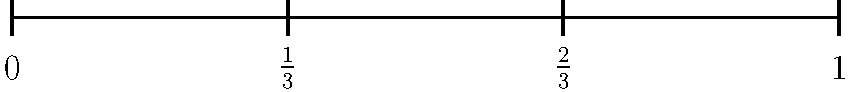
\includegraphics[]{3del}
\end{figure}\vspace{40pt}

\begin{figure}
	\centering
	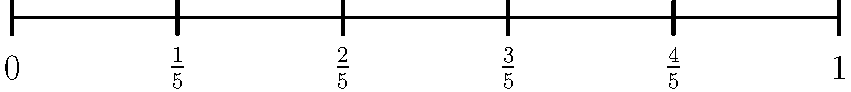
\includegraphics[]{5del}
\end{figure}\vspace{40pt}

\begin{figure}
	\centering
	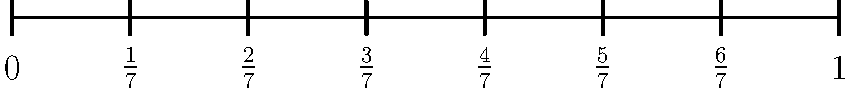
\includegraphics[]{7del}
\end{figure}\vspace{40pt}

\begin{figure}
	\centering
	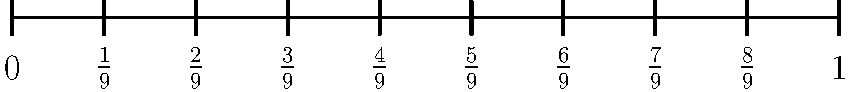
\includegraphics[]{9del}
\end{figure}\vspace{40pt}
\begin{figure}
	\centering
	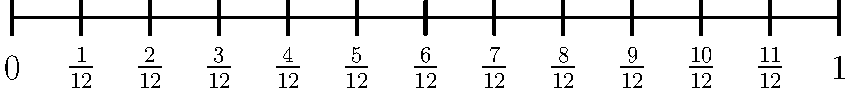
\includegraphics[]{12del}
\end{figure} \vspace{40pt}
\begin{figure}
	\centering
	
\includegraphics[]{4delb}
\end{figure} 

\end{document}